\section{Study Results}
\subsection{Objectives}
In order to assess the feasbility of extending the KCFN inside the UNI footprint,
it is essential to define well-established targets for any potential work. The
proposal that follows is intended to satisfy the following requirements:
\begin{description}
\item[Purpose] This proposal is for a project intended to improve the state of
connectvity for businesses and residents within the urban core, establish
local hubs for connectivity and digital skills
education, and demonstrate an organizing model that can be replicated in other
 communities.
\item[Scope] The geographical area under consideration is bounded by 22\textsuperscript{nd}
Street on the North, 71 Highway on the East, 52\textsuperscript{nd} Street on the South, and
Troost Avenue on the West. In addition to The UNI and UNI Partner organizations, it 
should involve an array of area residents, businesses, non-profits, and community groups.
\item[Coverage] The paramount concern is improving the availability of 
affordable residential Internet service for those within the designated geographic
scope. While it isn't possible to guarantee coverage to 100\% of residences with a community network approach,
our objective should be to allow any and all blocks within the area to participate. This
will not be possible without significant investment and involvement from within the
community itself.
\item[Functionality] Those that elect to participate in the network, in addition
to gaining access to resouces published on the KCFN, should have the
ability to purchase low-cost Internet access. 
\item[Performance] While exact performance figures will depend case-by-case on a
number of factors, the KCFN should enable broadband connectivity capable of supporting
telephony, web 2.0, and multimedia applications.
\item[Cost] The total cost of
accessing the Internet via the KCFN, including hardware, should be lower than existing
alternatives over the course of one year.
\item[Sustainibility] Above all, this effort should aim to foster a digital commons
that is sustainable in the long term --- focusing first and foremost on education, grassroots
support, and the capacity for ongoing, organic growth.
\end{description}
\subsection{Survey Information}
The primary physical considerations in determining build feasibility and an
appropriate course of action are topographic terrain, available structures, and the RF environment. 
We surveyed the target area in November and December of 2013, and January of 2014,
 analyzing the lay of the land and assesing spectrum availability. \par
\subsubsection{Overall Terrain}
The terrain in question is varied in topology and foliage density, and large enough
to make the use of a single, homogeneous network architecture impractical. As such,
we have divided the area into eight distinct `clouds'. These clouds do not conform
to existing neighborhood boundaries, but are instead focused on producing an efficient 
and cost-effective organizational scheme for the network.   
\begin{center}
\fbox{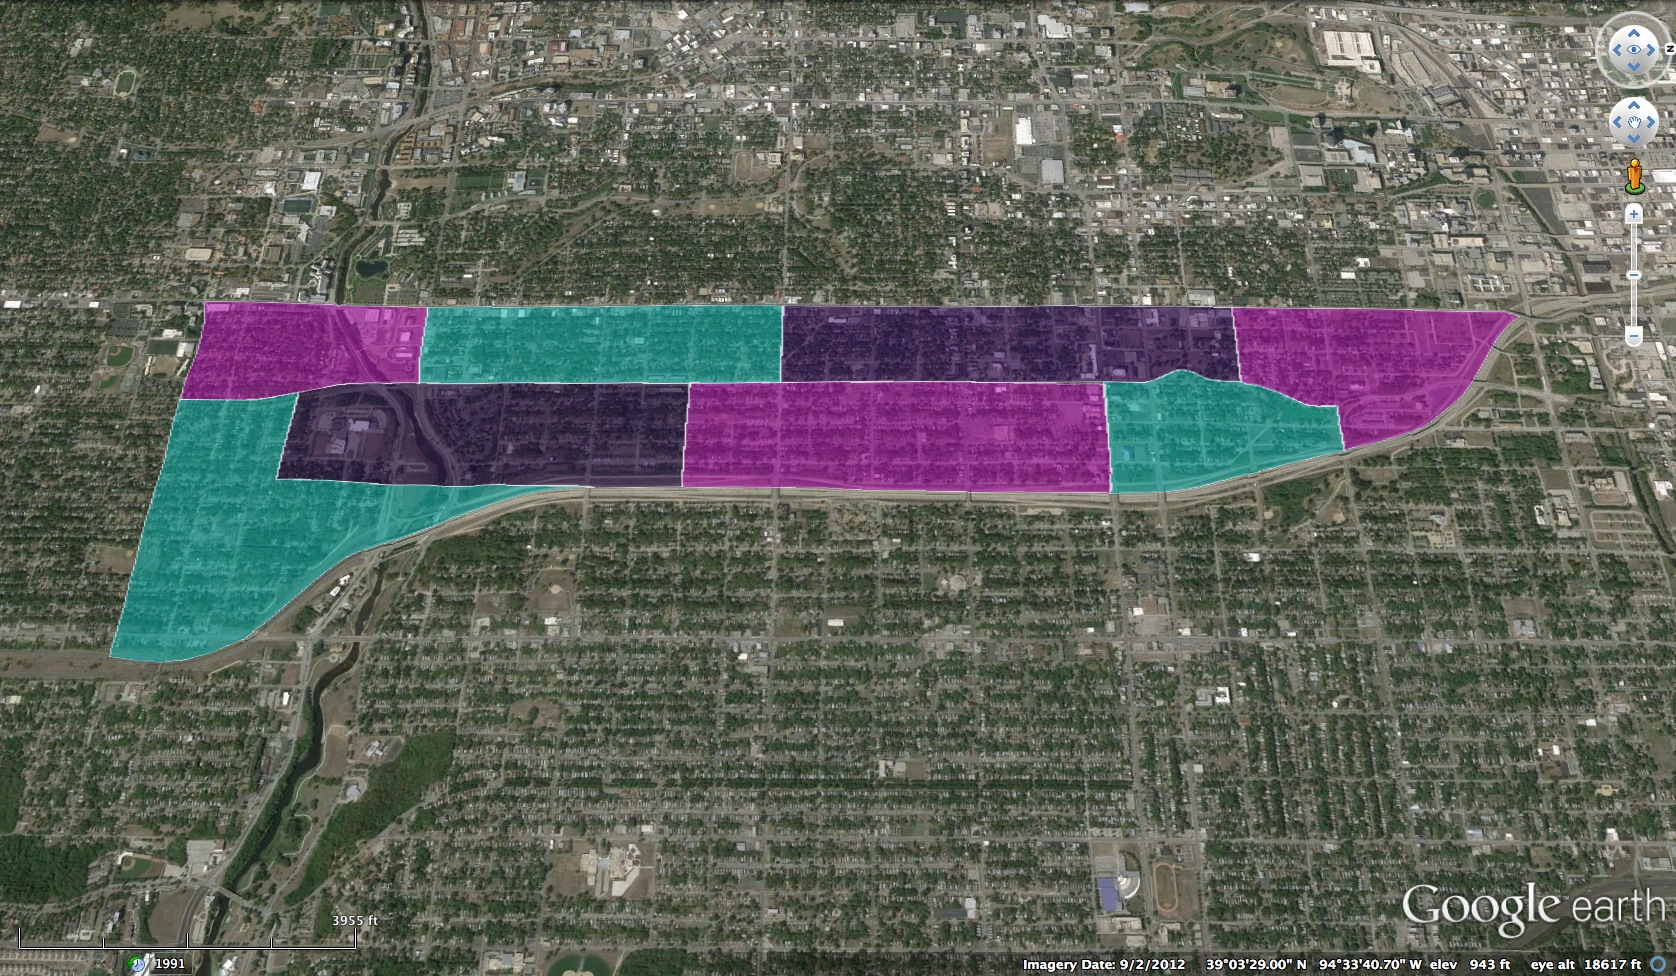
\includegraphics[width=5in]{clouds.jpg}}
\end{center}
The eight clouds, as depicted in the map above, are as follows:
\begin{description}
\item[Kelly Cloud] The Kelly Cloud presents the most difficult terrain in the study
area, with a significant rise in elevation to the west of 71 Highway, large foliage,
and few commercial structures. The Kelly Center provides sight lines to the eastern
face of Blue Hills, but a higher than usual density of relays will be required to 
achieve desired levels of coverage, especially in the ravine near 48\textsuperscript{th}
\& Brooklyn.
\item[Rockhurst Cloud] While the Rockhurst cloud has a similar dearth of viable commercial
relay sites, the terrain is more forgiving. Decent lines of sight should be achievable at
street level, requiring roughly 2 relays per block.
\item[Paseo Cloud] The Paseo cloud presents extremely favorable conditions. Paseo Academy's
commanding vista offers good coverage of the slight slope that rises north from Cleaver II Boulevard.
Slightly thinner than average tree cover will aid in establishing relays. 
\item[Bancroft Cloud] While the Bancroft cloud does not have many useful multi-story buildings,
the terrain is relatively forgiving. Despite steep gradients running East to West, longer relay
connections should be acheivable running South-North along major thoroughfares.
\item[Eastern Cloud] In the Eastern cloud, there are fewer steep gradients, and a decent number
of valuable relay sites. Slightly lower than average relay density should be achievable.
\item[St. Mary's Cloud] In St. Mary's cloud, there are a large number of commercial buildings,
with ample opportunities for interconnection. Relays will primarily communicate above tree level
here, and sepctrum management will be a key factor. A higher density of multi-dwelling units will
result in a higher ratio of relays to nodes.
\item[Mt. Hope Cloud] The Mt. Hope cloud, like the Rockhurst Cloud, will need approximately two
relays per block. This is due to slight but considerable slopes, and a lack of prominent edifices.
\item[Beacon Cloud] Presuming the availablity of high-rise structures on West Paseo, the Beacon cloud
should be relatively easy to cover. These high-rise structure, situated on a relatively open plain,
will reduce the need for block-level relays.
\end{description}

\subsubsection{Structures}
While terrain is certainly key, it must be coupled with a knowledge of which structures are
suitable for the placement of equipment. Numerous factors affect the suitability of a structure,
include its location, height, roof architecture, constructure, and usage.
The map below illustrates how an ideal tower-to-tower network would be arranged:
\begin{center}
\fbox{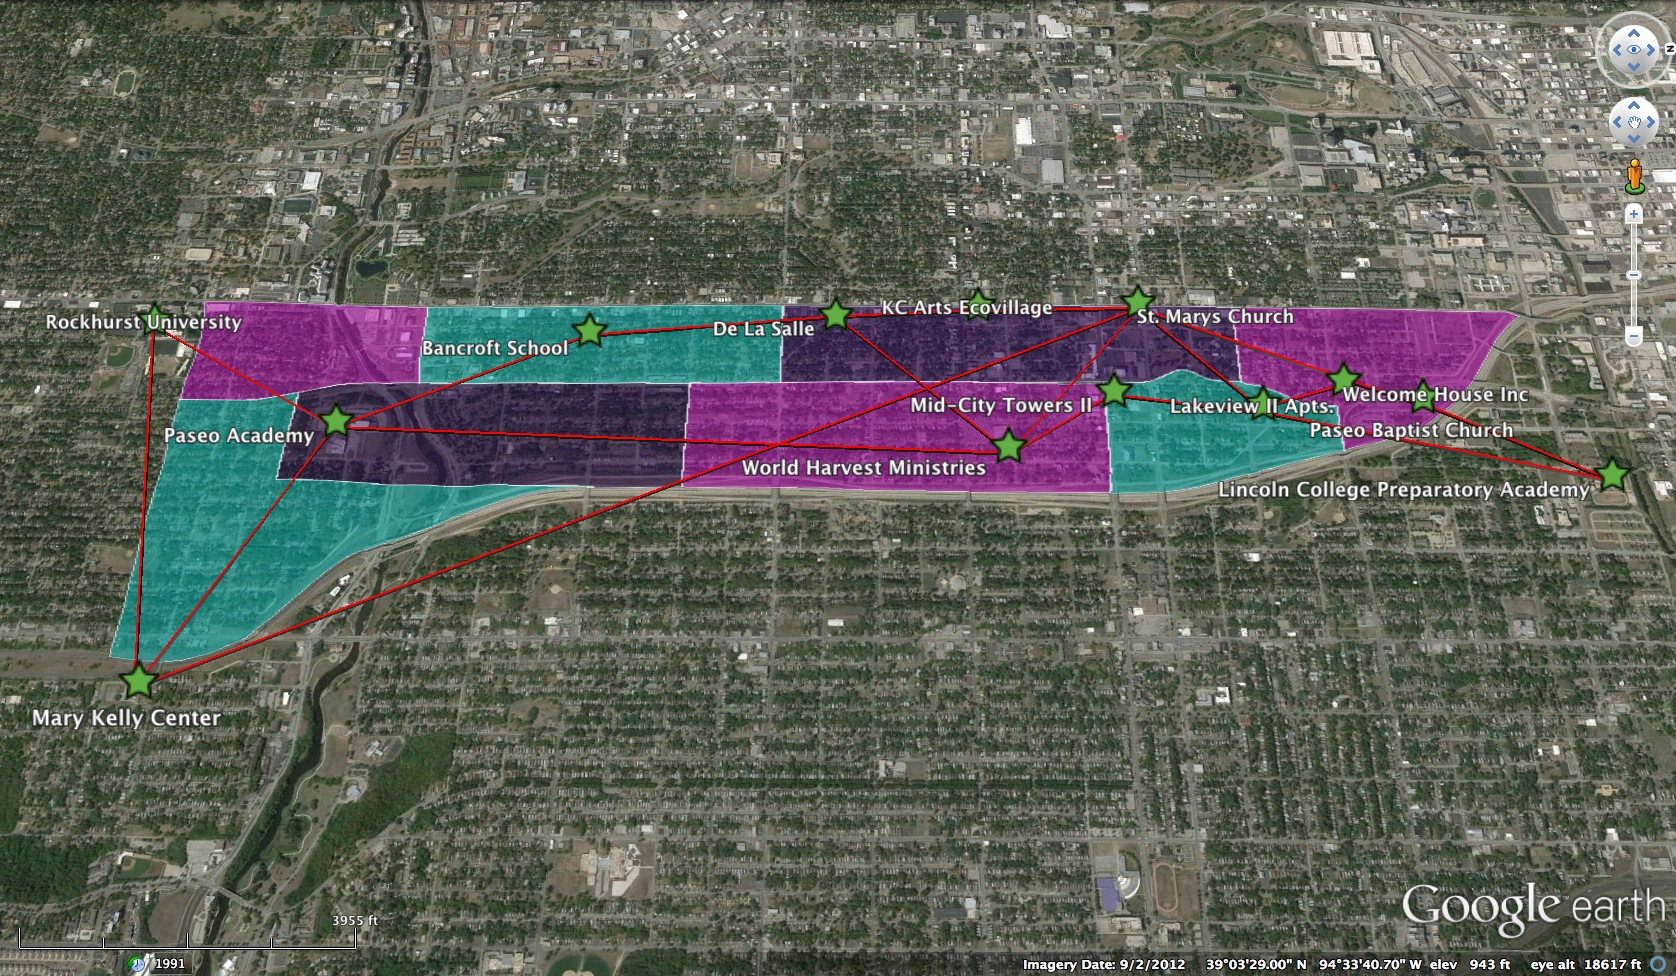
\includegraphics[width=5in]{towers.jpg}}
\end{center}
While we have determined these sites as the ideal tower placements, we
understand that the facts on the ground in each neighborhood will inform final selection of
locations.\par
In addition to surveying the entire study footprint for tower locations, we conducted detailed
studies of the St. Mary's and Mt. Hope clouds. These detailed studies were used to create the
projections of cost presented in our findings. The following map depicts a proposed distribution
of relays across two of the clouds:
\begin{center}
\fbox{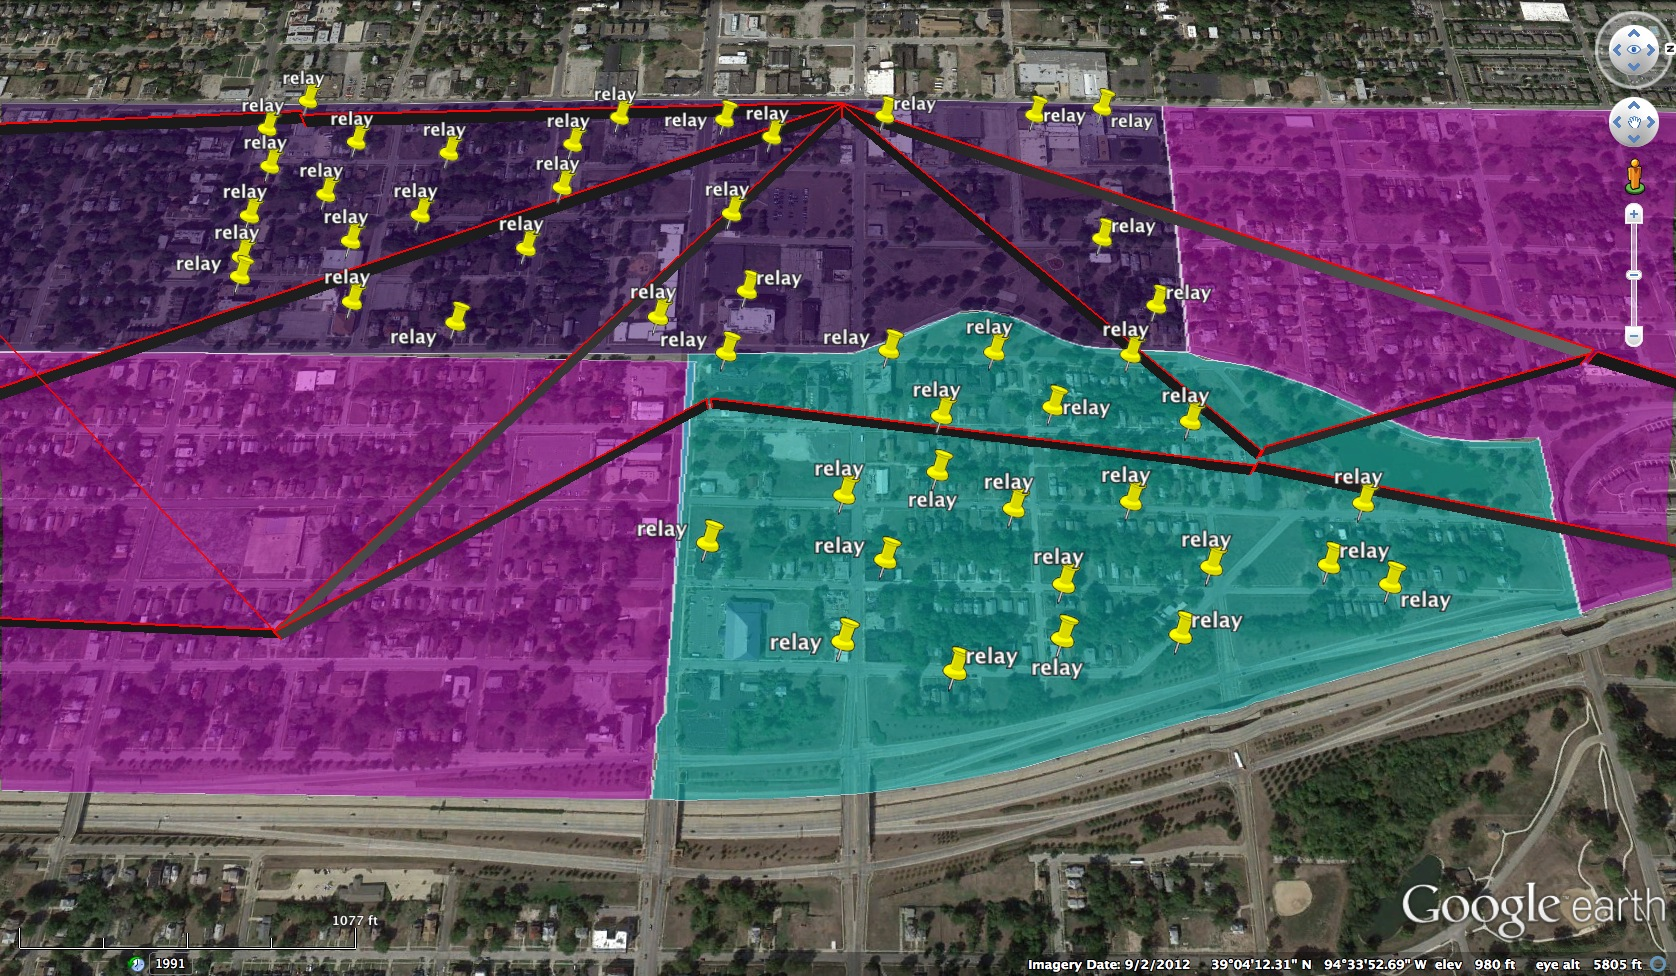
\includegraphics[width=5in]{relays.jpg}}
\end{center}

\subsubsection{RF Environment}

Our finding is that while appropriate channel selection and efficiency will be critical,
there is ample spectrum available for use in the target geography. In order to
assess spectrum health, we conducted sector surveys from the roof of St. Mary's, at 31\textsuperscript{st}
\& Troost, and the Kelly Center at 51\textsuperscript{st} \& Chestnut. Looking to the north of St. Mary's,
there is more than 50MHz of usable spectrum:\par
\begin{center}
\fbox{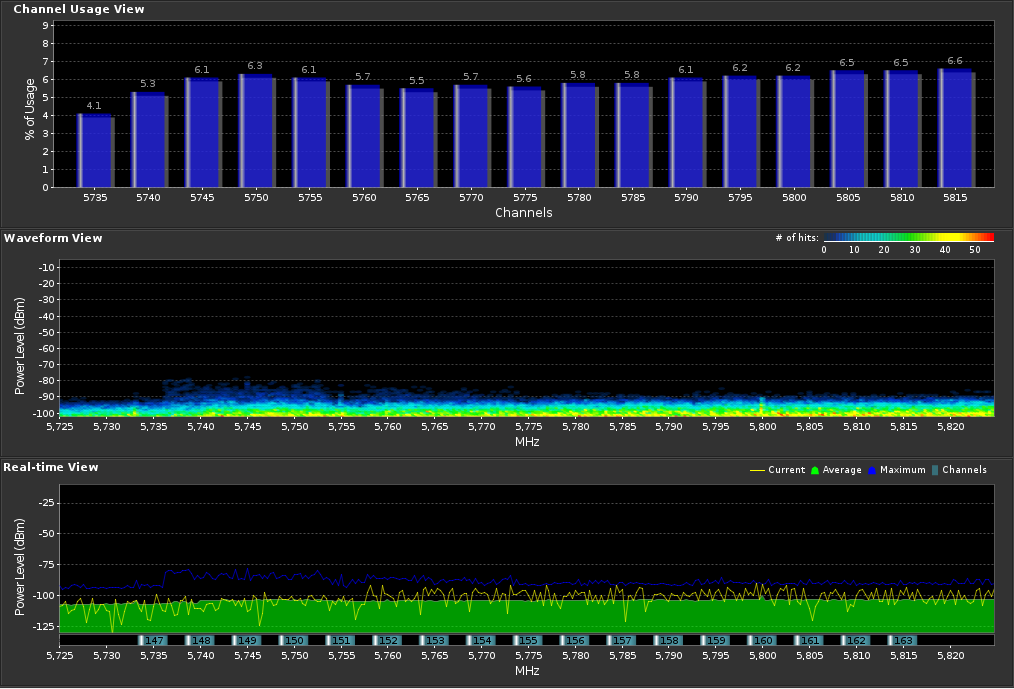
\includegraphics[width=4in]{stmnorth.png}}
\end{center}
To the east of St. Mary's 75MHz is usable, with a noise floor below 90dBi. This is enough spectrum
for three or four high throughput point-to-point links:
\begin{center}
\fbox{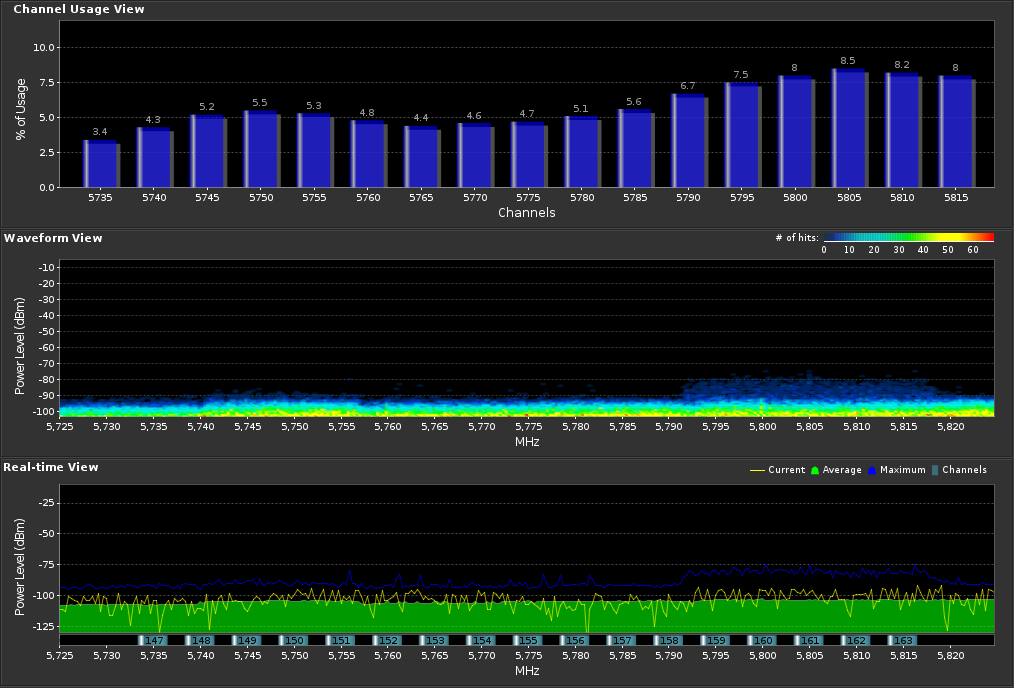
\includegraphics[width=4.5in]{stmeast.png}}
\end{center}
To the south of St. Mary's there is 65MHz of clean, usable spectrum, which should be more than enough
to build the requisite links:
\begin{center}
\fbox{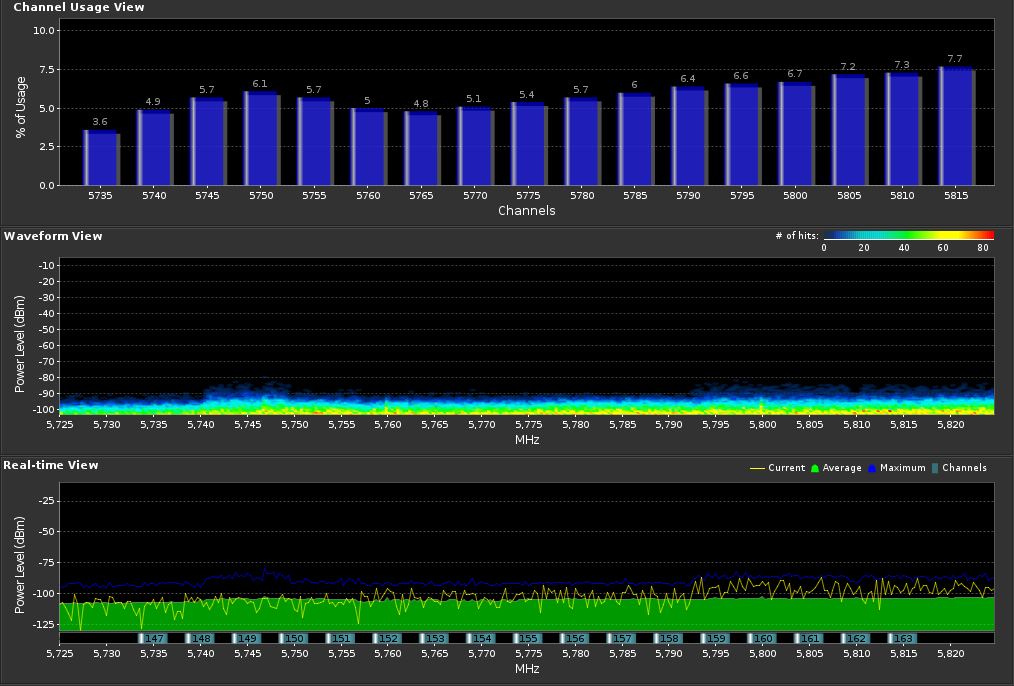
\includegraphics[width=4.5in]{stmsouth.png}}
\end{center}
At the southern end of the study area, the situation looks quite similar, though
with a slightly higher thermal floor. Looking north from the Kelly Center, there
is 70MHz available:
\begin{center}
\fbox{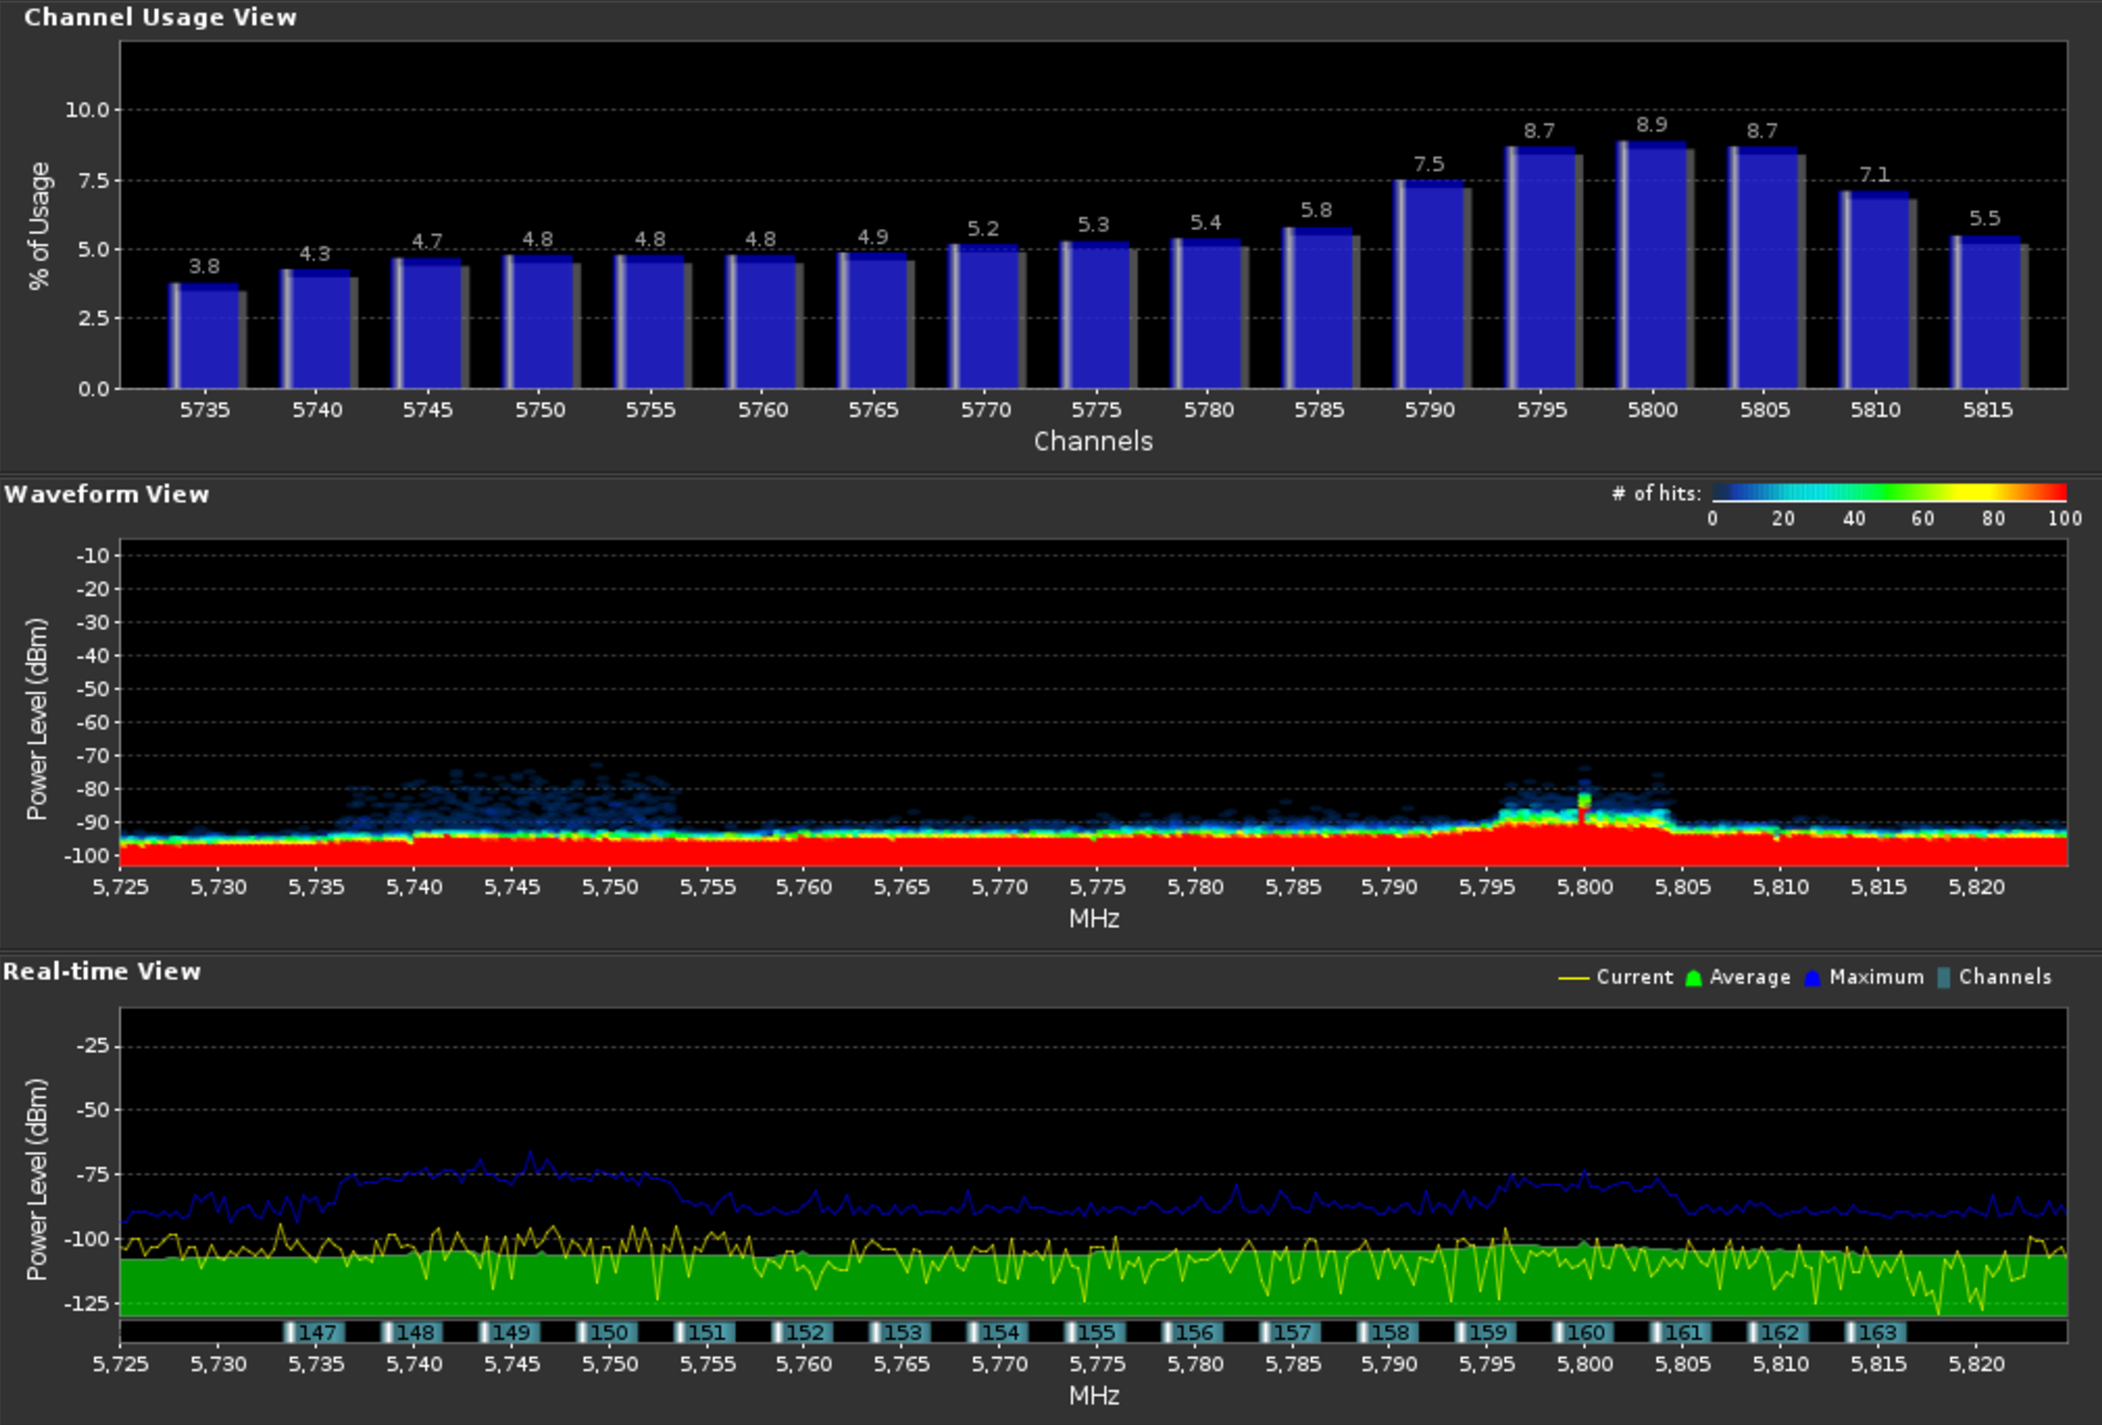
\includegraphics[width=4.5in]{to3101_rf_airview_crop.pdf}}
\end{center}
Looking west from the Kelly center, towards Blue Hills and some of the most challenging terrain,
virtually the entire 5GHz ISM band is available:
\begin{center}
\fbox{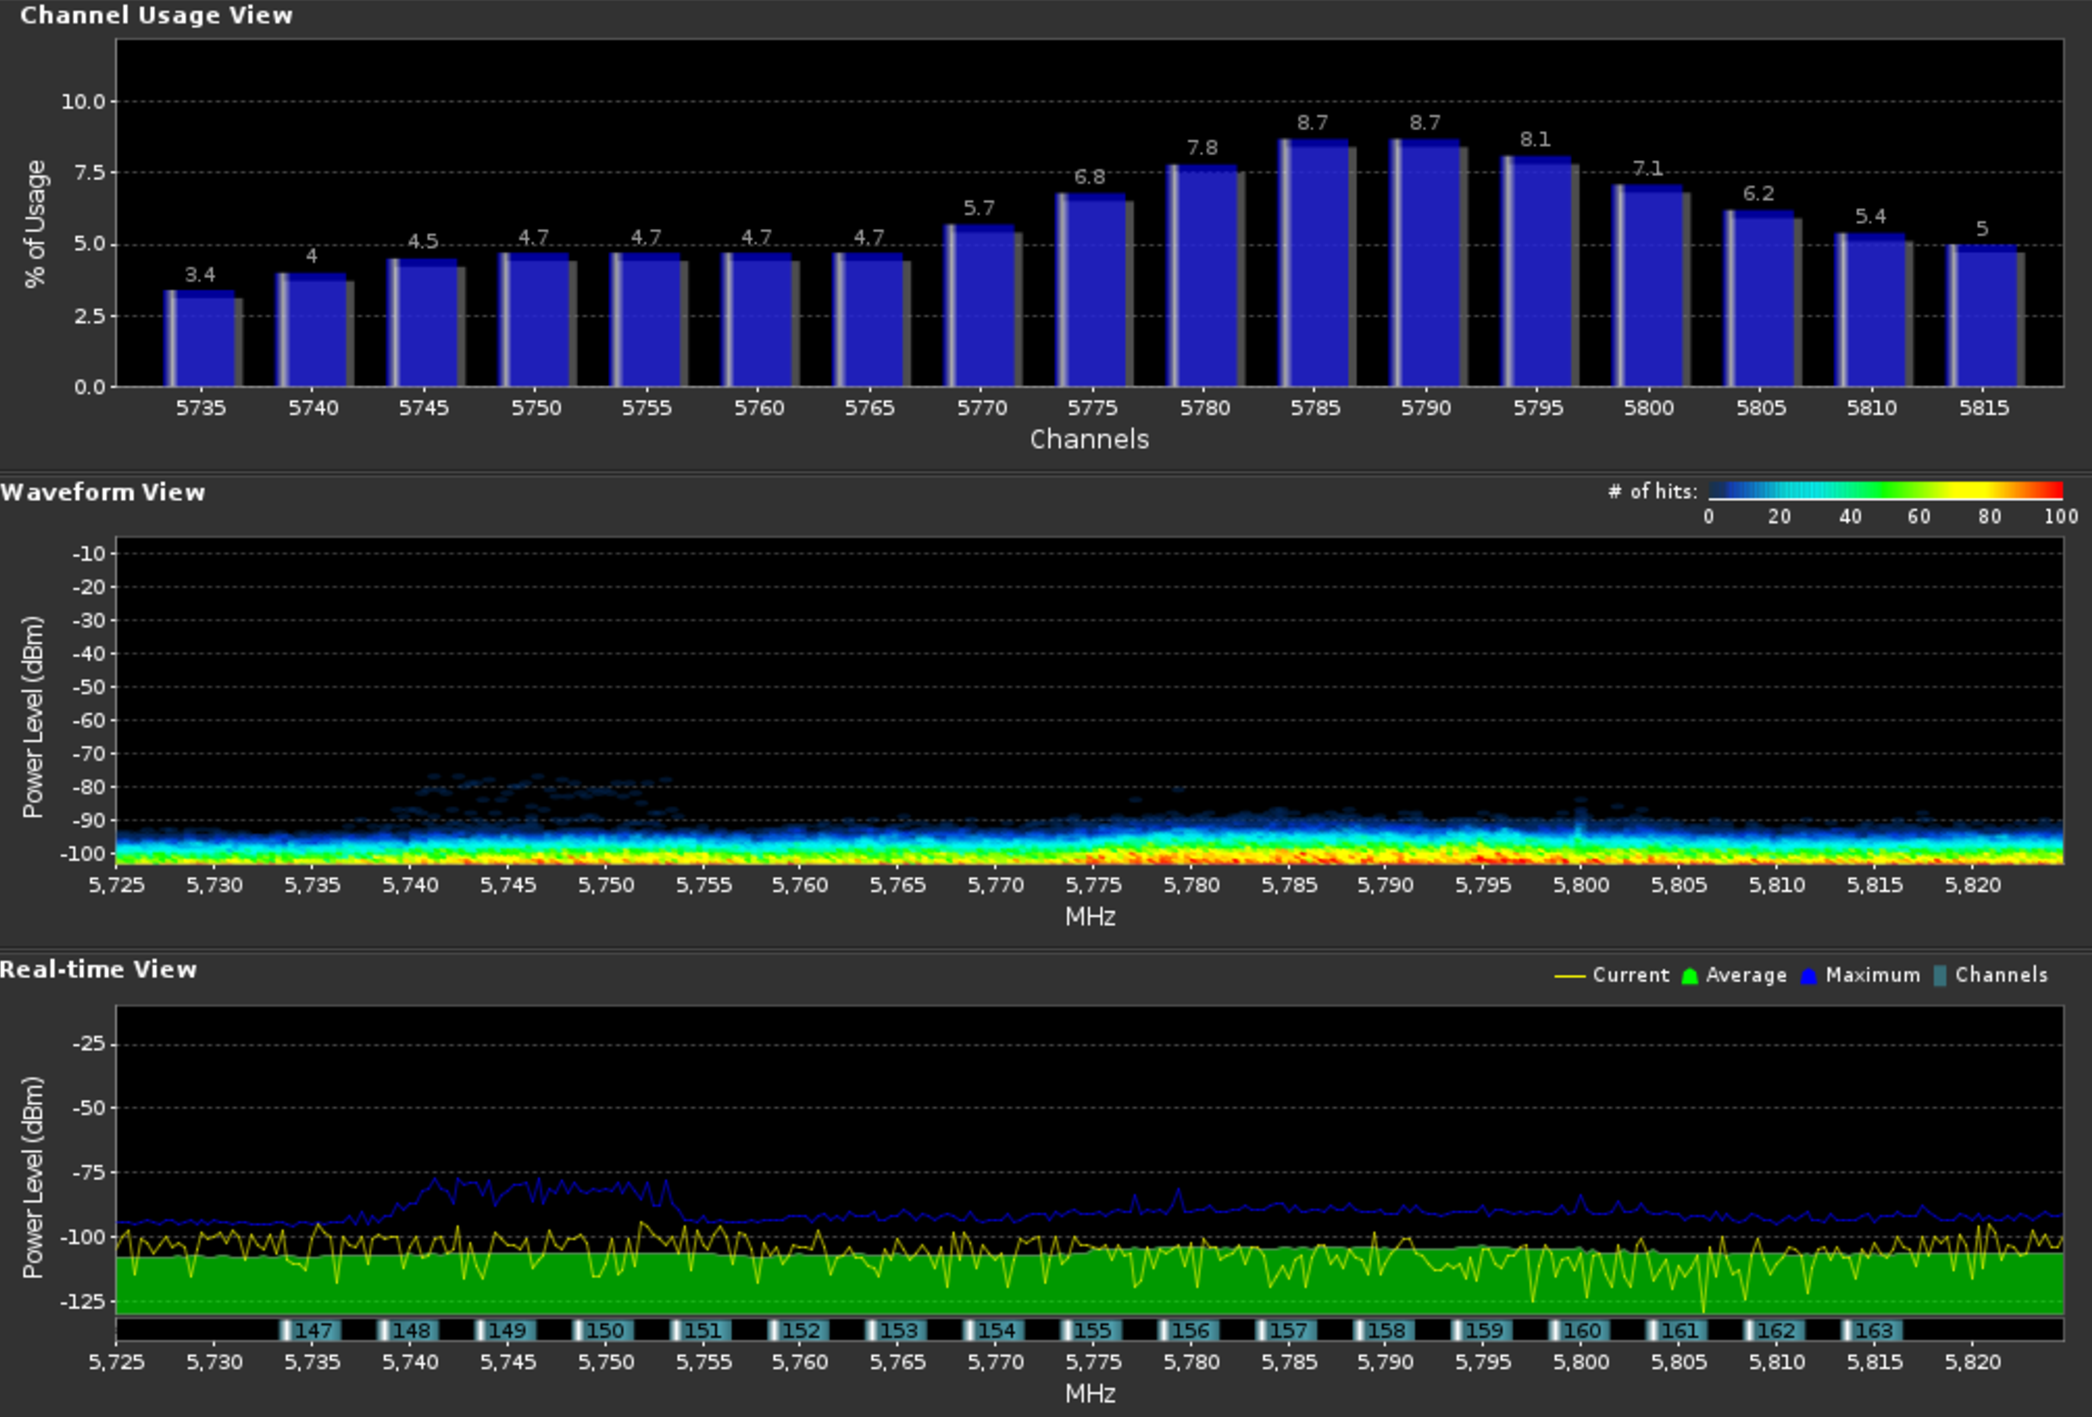
\includegraphics[width=4.5in]{due_west_airview_crop.pdf}}
\end{center}
\subsection{Social \& Political Considerations}
Though the laws of physics are unbending, they are certainly less complex than the laws of
human interaction. Over the past several months, we have reached out to community leaders
to guage interest in the project of building a network for and by the community. Those leaders
include Margaret May, Mark Stalsworth, Wanda Taylor, Jonathon Bish, Joanne Bushinger, and
decision makers at Kansas City Public Schools, and Kansas City Public Libraries. We have
received promising indications of future partnership from all. \par
There will doubtlessly be further planning and exploration as we move forward, in order to
assure that all parties have a sound understanding of the obstacles and opportunties afforded
by this endeavour. Community organizing will be the bulk of the work in building a network,
and we are confident that these and other partners are more than up to the task.

\subsection{Findings}
On the basis of our survey results and prior field experience, we have devised
a proposed plan of action and associated cost estimates. These projections are intended
to serve as a starting point for collaboration, and certainly do not reflect the
only viable path towards accomplishing the stated objectives.\par
\subsubsection{Proposed Plan}
\begin{description}
\item[Phase 0 - Q1,2 2014] Improvements to the network, including the construction of a high-speed backbone,
fully fault-tolerant routing, and robust user authentication are slated for completion in the first half of
2014. This should provide lead time for the UNI and UNI partners to organize programming around the network.
More than raising capital for Phase I construction projects, we advise focusing on community outreach and
education: building teams, and beginning to identify network operators.
\item[Phase I - Q3,4 2014] Once the current round of network improvements is implemented, the first clouds
should begin to come online. We have identified the St. Mary's and Bancroft clouds as the ideal
locales for pilot work. Phase I would involve a concerted effort to raise public awareness of the network,
construction of a FreedomTower for the Bancroft cloud, and the initial rollout of relays and nodes in the indicated
areas. \par
Connecting for Good and Free Network Foundation engineers, rather than directly building and operating the networks,
should be regarded mainly in an advisory role: training operators, and supervising the rollout.
\item[Phase II - 2015]  In Phase II, all remaining clouds should come online, while established ones proliferate and
achieve desired coverage levels. CFG and FNF would continue to play a supporting role, ensuring continuity of
operation of core infrastructure, but the onus of neighborhood network operation should be squarely on the community
itself.
\item[Phase III - 2016 \& Beyond] Once the initial rollout of the network is complete, focus should shift entirely
to sustaining the effort. Responsibility for core infrastructure should be shared with or transferred to proven community
operators. Training future operators and network participants will become the responsibility of network participants, along
with Connecting for Good. The Free Network Foundation will serve only as an as-needed resource for solving high-level
technical issues. The network, at this point, should be a point of pride for the community, and very much viewed as
a cooperative, participatory effort.
\end{description}

\subsubsection{Costs}
While the community-driven model has its definite strengths, it can also make it difficult to give precise estimates of cost. 
Below, we provide the hard costs associated with building various network components, and estimates of the total number of
such devices that would be required to achieve full coverage in each of the eight network clouds.\par

FreedomTower:
\begin{center}
\begin{tabular}{|p{5cm}|l|l|l|}
\hline
Item & Q'ty Req'd & Unit Cost & Total Cost \\ \hline
Ubiquiti ToughCable & 2000ft & \$.22/ft & \$220 \\ \hline
Ubiquiti ToughConnectors & 20 & \$.53 & \$10.60 \\ \hline
Ubiquiti ToughSwitch-8 & 1 & \$188 & \$188 \\ \hline
Ubiquiti Rocket M5 & 5 & \$85 & \$425 \\ \hline
Ubiquiti RocketDish 5G30 & 2 & \$150 & \$300 \\ \hline
Ubiquiti Sector 5G19-120 & 3 & \$140 & \$420 \\ \hline
3-Gang Cluster Mount & 1 & \$131 & \$131 \\ \hline
Alix 2D13 Router & 1 & \$139 & \$139 \\ \hline
Rohn-25GBRM Mount & 1 & \$1458 & \$1458 \\ \hline
Rohn-BRM6PAD Insulator & 1 & \$360.90 & \$360.90 \\ \hline
Rohn-LRCL Arrest & 2 & \$123 & \$246 \\ \hline
\#4 Copper Wire & 40' & \$1.69/ft  & \$67.60 \\ \hline
Rohn-25G Tower Section & 2 & \$117.95 & \$235.90 \\ \hline
Labor & 75hr & \$75 & \$ 3750 \\ \hline
Total & - & - & \$7,952 \\ \hline
\end{tabular}
\end{center}

FreedomRelay:
\begin{center}
\begin{tabular}{|p{5cm}|l|l|l|}
\hline
Item & Q'ty Req'd & Unit Cost & Total Cost \\ \hline
Ubqiuiti ToughCable & 500ft & \$.22/ft & \$55 \\ \hline
Alix 2D2 Router & 1 & \$110 & \$110 \\ \hline
Alix 2C4 Enclosure & 1 & \$60 & \$60 \\ \hline
Ubiquiti SR71-15 & 2 & \$85.99 & \$171.98 \\ \hline
L-Com HG5808U Antenna & 4 &  \$78.95 & \$315.80 \\ \hline 
Laird SMA Adapter & 4 & \$7.75 & \$31 \\ \hline
Passive PoE Adapter & 1 & \$3.50 & \$3.50 \\ \hline
Alix BRK1D Mount & 1 & \$2.50 & \$2.50 \\ \hline
Labor & 2hr & \$50 & \$100 \\ \hline
Total & - & - & \$849.78 \\ \hline
\end{tabular}
\end{center}

FreedomNode:
\begin{center}
\begin{tabular}{|p{5cm}|l|l|l|}
\hline
Item & Q'ty Req'd & Unit Cost & Total Cost \\ \hline
Netgear WNDR3800 & 1 & \$114.99 & \$114.99 \\ \hline
Labor & 1hr & \$25 & \$25 \\ \hline
Total & - & - & \$139.99 \\ \hline
\end{tabular}
\end{center}

Based on the cost figures above, and the density, terrain, extant structures,
foliage, and RF environment encountered in our survey, we project the following
costs to achieve full coverage of the entire UNI footprint:

\begin{center}
\begin{tabular}{|p{3cm}|l|l|l|l|}
\hline
  & Towers & Relays & Nodes & Total \\ \hline
Kelly & 1 & 55 & 400 & 456 \\ \hline
  & \$7,952 & \$46,737.90 & \$55,596 & \$110,285.90 \\ \hline
Rockhurst & 1 & 48 & 300 & 349 \\ \hline
  & \$7,952 & \$40,789.44 & \$41,997 & \$90,738.44 \\ \hline
Paseo & 1 & 35 & 250 & 386 \\ \hline
  & \$7,952 & \$29,742.30 & \$34,997.50 & \$72,691.80 \\ \hline
Bancroft & 1 & 55 & 400 & 456 \\ \hline
  & \$7,952 & \$46,737.90 & \$55,996 & \$110,685.90 \\ \hline
Eastern & 1 & 46 & 500 & 547 \\ \hline
  & \$7,952 & \$39,089.88 & \$69,995 & \$117,036.88 \\ \hline
St. Mary's & 2 & 65 & 300 & 366 \\ \hline
  & \$15,904 & \$55,235.70 & \$41,997 & \$113,136.70 \\ \hline
Mt. Hope & 2 & 49 & 310 & 360 \\ \hline
  & \$15,904 & \$41,639.22 & \$43,396.90 & \$100,940.12 \\ \hline
Beacon & 1 & 30 & 200 & 231 \\ \hline
  & \$7,952 & \$25,493.40 & \$27,998 & \$61,443.40 \\ \hline
Totals & 10 & 383 & 2,660 & 3,053 \\ \hline
  & \$79,520 & \$325,465.74 & \$372,373.40 & \$777,359.14 \\ \hline
\end{tabular}
\end{center}

In looking at these numbers, it is important to keep in mind that for the network to 
succeed, as much of the capital investment as possible should come from the community
itself. Outside support, if utilized, should be limited to funding initial tower builds,
to seed organic, internal growth. \par
Organizational support should focus on outreach and education, with the aim of producing
a corps of capable network operators from inside the community. Aside from create jobs,
this approach fosters a self-sufficient and sustainable network that does not depend on
any single entity.
